\chapter{Uzi koordinatojn}
\label{koordinatoj}

{ }\hfill\textbf{Nivelo:} komencanto
\section{Prezentado}
\noindent En tiu ^ci ^capitro, ni malkovros la primitivon
\texttt{situon\_provizu}.  La desegnareo havas dratreton kies origino
estas lokita je la centro de la ekrano.  Oni povas atingi ^ciun
punkton de la desegnejo per helpo de ^giaj koordinatoj.

\texttt{sitp listo}\hspace {4cm } \textcolor{red}{ \texttt{sitp [100 -250]}}\\
Movas la testudon al la punkto kies koordinatojn difinas la listo.\\ \\
\\ Malgranda uzekzemplo:\\
\texttt{ev sitp [200 100] sitp [50 -150] sitp [-100 -150]}
\begin{center}
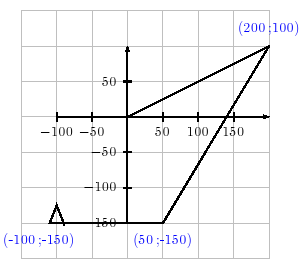
\includegraphics[scale=0.7]{bildoj/fpos-coord.png}
\end{center}
\vspace{1cm}
\section{Ekzerco:}
\noindent
Realigu tiun figuron nur uzante la primitivojn: \texttt{sitp}, \texttt{ev}, \texttt{l}, \texttt{ml}.\\
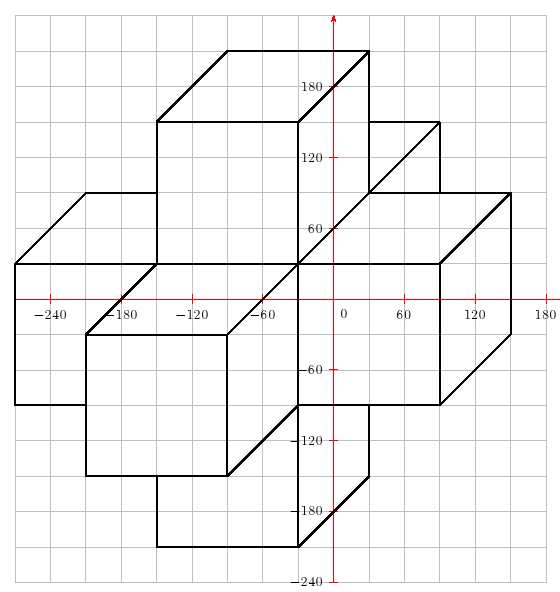
\includegraphics[scale=0.7]{bildoj/fpos-cube.png}
